%\documentclass[a4paper,twoside,10pt]{article}
\interfootnotelinepenalty=10000
\usepackage[USenglish]{babel} %francais, polish, spanish, ...
\usepackage[T1]{fontenc}
%\usepackage[ansinew]{inputenc}
\usepackage{color}
\usepackage{mathtools}
%\usepackage{hyperref}
\usepackage{subfig}
\usepackage{multirow, booktabs}
\usepackage{hyperref}


\usepackage{lmodern} %Type1-font for non-english texts and characters
\usepackage{algorithm}
\usepackage[noend]{algpseudocode}
\usepackage{mnsymbol}

%% Packages for Graphics & Figures %%%%%%%%%%%%%%%%%%%%%%%%%%
\usepackage{graphicx} %%For loading graphic files
\usepackage{amsmath}
\usepackage{amsthm} 
\usepackage{thmtools}
\usepackage{amsfonts}
\usepackage[all,cmtip]{xy}
\usepackage{tikz}

\usepackage{TechFront}
%\declaretheorem{Lemma}
%\declaretheorem{prop}

\newcommand{\lre}{\color{red}{\{}}

%\DeclareMathOperator{\sign}{sgn}
%\DeclareMathOperator{\coef}{coef}
%\DeclareMathOperator{\var}{var}
%\DeclareMathOperator{\eqs}{eqs}
%\DeclareMathOperator{\feas}{feas}
%\DeclareMathOperator{\UB}{UB}
%\DeclareMathOperator{\lb}{lb}
%\DeclareMathOperator{\FMcomb}{FM-comb}
%\DeclareMathOperator{\Gcomb}{Gauss-comb}
%\DeclareMathOperator{\proj}{proj}
%\DeclareMathOperator{\Pos}{Pos}
%\DeclareMathOperator{\Neg}{Neg}
%\DeclareMathOperator{\rhs}{rhs}
\newcommand{\sign}{\mathit{sgn}}
\newcommand{\coef}{\mathit{co}}
\newcommand{\var}{\mathit{var}}
\newcommand{\VAR}{\mathit{VAR}}
\newcommand{\eqs}{\mathit{eqs}}
\newcommand{\feas}{\mathit{feas}}
\newcommand{\UB}{\mathit{UB}}
\newcommand{\UBc}{\mathit{UBineq}}
\newcommand{\lb}{\mathit{lb}}
\newcommand{\lbc}{\mathit{lbineq}}
\newcommand{\FMcomb}{\mathit{FM}}
\newcommand{\Gcomb}{\mathit{GA}}
\newcommand{\proj}{\mathit{proj}}
\newcommand{\Pos}{\mathit{Pos}}
\newcommand{\Neg}{\mathit{Neg}}
\newcommand{\rhs}{\mathit{rhs}}
\newcommand{\bounds}{\mathit{bounds}}
\newcommand{\ie}{\mathcal{IE}}
\newcommand{\xx}{\mathcal{X}}
\newcommand{\vea}{\mathbf{co}}
\newcommand{\ttt}{\texttt{t}}
\newcommand{\trt}[1]{\texttt{#1}}
\newcommand{\mi}{\mathit}

\newcommand{\false}{\texttt{false}}
\newcommand{\true}{\texttt{true}}
\newcommand{\nul}{\texttt{null}}
\newcommand{\ve}{\mathbf}
%\newcommand\lhs[1]{\text{lhs}(#1)}
%\newcommand\rhs[1]{\text{rhs}(#1)}
%\newcommand\coef[1]{\text{coef}(#1)}
%\newcommand\LB[1]{\text{LB}_{#1}}
%\newcommand\UB[1]{\text{UB}_{#1}}
\newcommand{\lig}[4]{\ve{#1}\cdot\ve{#2}#3#4}
\newcommand\red[1]{\textcolor{red}{#1}}
\newcommand\blue[1]{\textcolor{blue}{#1}}
\newcommand{\set}[2]{\{\;{#1}\;|\;{#2}\;\}}
\newcommand{\odef}{\overset{\text{def.}}=}
\newcommand{\mc}{\mathcal}
\algdef{SE}[DOWHILE]{Do}{doWhile}{\algorithmicdo}[1]{\algorithmicwhile\ #1}%
\newcommand{\argmin}{\operatornamewithlimits{argmin}}
\newcommand{\StateInd}{\State\hspace{\algorithmicindent}}
\newcommand{\pr}{\mathit{PR}}
\newcommand{\prs}{\mathit{PRS}}
\newcommand{\ens}{\Leftrightarrow}

%\algdef{SE}[DOPAR]{DoPar}{doParWhile}{\algorithmicdo\textbf{ in parallel for\ }}[1]{\algorithmicwhile\ #1}%
\algdef{SE}[DOPAR]{DoPar}{doParUntil}{\algorithmicdo\textbf{ in parallel for\ }}[1]{\algorithmicuntil\ #1}%

\algdef{SE}[SUBALG]{Indent}{EndIndent}{}{\algorithmicend\ }%
\algtext*{Indent}
\algtext*{EndIndent}

\newtheorem{prop}{Proposition}
\newtheorem{lemma}{Lemma}
\newtheorem{cor}{Corollary}

\newcounter{para}
%\newcommand\mypara[1]{\par\refstepcounter{para}\textbf{\thep‌​ara\space#1\space}}
\newcommand\mypara[1]{\newline\par\refstepcounter{para}\textbf{\thepara}\space \textbf{#1} \space}
%\newcommand\mypara{\par\refstepcounter{para}\thepara\space}
%\usepackage[thmmarks,...]{ntheorem}
\newcommand{\Sec}{F}
\newcommand{\Ca}{\mi{Cap}}
\newcommand{\Vol}{\mi{V}}
\newcommand{\Weight}{\mi{W}}
\newcommand{\weight}{\mi{w}}
\newcommand{\BonjeanStations}{\mi{BS}}
\newcommand{\bonjean}{bf}
\newcommand{\Bonj}{B}
\newcommand{\shear}{\mi{sf}}
\newcommand{\Prop}{P}

\theoremstyle{definition}
%\newtheorem{example}{Example}[section]
\newtheorem*{theorem}{Theorem}

\theoremstyle{definition}
\newtheorem{examplex}{Example}[section]
\newenvironment{example}
  {\pushQED{\qed}\renewcommand{\qedsymbol}{$\triangle$}\examplex}
  {\popQED\endexamplex}
	
%\newtheoremstyle{named}{}{}{\itshape}{}{\bfseries}{.}{.5em}{\thmnote{#3}}
%\theoremstyle{named}
%\newtheorem*{namedtheorem}{Theorem}


%\begin{document}
\section{Vessel Model}
In this section we will describe the data given for a stowage model, and we will explain how this information is translated into our proposed \emph{Vessel Model} (VM).

The main purpose of our VM is to 
{describe the hydrostatic constraints reasonably accurate while}
abstracting away much of the unnecessary complexity relating to the physical layout of the vessel. 
More specifically, the buoyancy data used in hydrostatic calculations are given at a set of points along the vessel (stations), while hydrostatic constraints are given in relation to another set of points (frames), and neither of these coincide with the position of the structures holding the cargo or the ballast tanks (see Figure~\ref{fig:vessel}). The measure points are aligned in the VM, and calculations for the hydrostatic constraints are simplified (see Figure~\ref{fig:sectionEndPoints}).

The data used as input to the stowage models are real vessel profile files used by a professional loading computer. These vessel profiles have been kindly provided by our industrial partners.

\subsection*{Vessel data}
\paragraph{Vessel structure and container types}
The cargo space of a container vessel is divided into parts called \textit{bays} that each consists of a grid of \emph{cells}. Each cell is divided into two \emph{slots} and can accordingly hold one standard 40' container or two 20' containers. Some cells have power plugs allowing for \emph{reefer} containers to be refrigerated as required. Each bay is divided into three or four parts called \textit{locations}, at which level the vessel's capacities are given. See Figure~\ref{fig:vessel}.

\begin{figure}[hb]
	\centering
		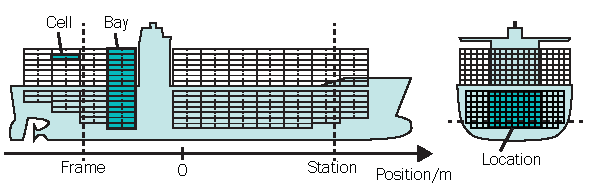
\includegraphics{figures/vessel2.pdf}
	\caption{(a) Vessel structure and reference points seen on a longitudinal intersection X, and (b) on a transversal intersection.}
	\label{fig:vessel}
\end{figure}

To define common reference points for cargo-holding structures and hydrostatic constraints, we further define larger \emph{sections} of the vessel and their endpoints. Each of these sections either span a number of succeeding bays, or a part of the ship containing no bays at all.
See Figure~\ref{fig:vessel} and Figure~\ref{fig:sectionEndPoints}.

\begin{figure}[hb]
	\centering
		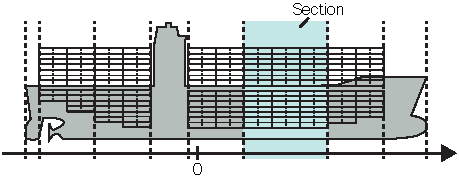
\includegraphics{figures/sectionEndPoints.pdf}
	\caption{Sections on a vessel. Their endpoints will be common reference points for cargo-holding structures and hydrostatic constraints in the VM.}
	\label{fig:sectionEndPoints}
\end{figure}

An empty vessel without cargo ballast or equipment is referred to as \emph{lightship}.  The lightship is given in the data by a set of ``blocks'' placed along the vessel. Each block has a given weight that is assumed to be equally distributed along the block.

The cargo itself is described by a container \emph{type}, which is defined by a length (20' or 40')\footnote{45' long containers are also common, but for the sake of simplicity, we only consider 20' and 40' containers in this article.}, whether it is a reefer-container or not, and a weight class (in a discrete set of weights). 
Besides containers, vessels also carry \emph{ballast tanks} in fixed positions along the vessel that can be filled with water to improve the stability of the vessel.

\paragraph{Capacities}
Though containers physically are placed in specific slots, the considered vessel data specifies capacities for each location. These capacities are given in \emph{TEU} (Twenty-foot Equivalent Units), i.e. a standard $20'$ container takes up one TEU, while a $40'$ container takes up two TEU. For each location, the vessel data includes upper bounds for: the total number of TEUs, $20'$ containers, $40'$ containers, reefer slots, reefer cells, plus separate total weight limit for $20'$ and $40'$ containers, respectively. The latter exist, since only $20'$ containers rest on the middle support posts of the stack it is in, while the end posts hold weight of both $20'$ and $40'$ containers. This may lead to different weight capacities of $20'$ and $40'$ containers.

Limits for each ballast tank are likewise given in the input data, as well as a limit for the total displacement, i.e. the weight of the vessel, including ballast water, cargo and the ship itself. 
%

\paragraph{Stress forces}
On a vessel, stress forces arise as a result of gravitation acting downwards and buoyancy acting upwards. This results in shear forces and bending moments along the longitudinal axis of the vessel, and limits on these are given for a set of reference points along the vessel called \emph{frames} (see Figure~\ref{fig:vessel}). 
%
The buoyancy force comes from the vessel's displacement of water and hence depends on the varying (and irregular) shape of the hull and the displacement of the vessel. The area submerged in water is given at another set of reference points called \emph{stations} for a discrete set of displacement values. See Figure~\ref{fig:vessel}.
It is the position of these reference points, that do not line up with bay endpoints, which is remedied in the VM.

Further requirements to ensure the stability of the vessel are imposed in real life and considered eg. in \cite{AlbertosThesis}, but is not considered here.

\paragraph{Input Data}
The vessel structure is described using the sets $L$ (locations), $BT$ (ballast tanks), $B$ (blocks with a constant weight $W_b$ for all $b\in B$), $ST$ (stations) and $F$ (frames). All elements in these sets have a fixed longitudinal position fore and aft ( $P^\trt{f}_e$ and $P^\trt{a}_e$ for all $e\in L\cup BT \cup B \cup ST \cup F$), and for the latter two sets, the fore and aft position coincide. %[For modeling purposes, an (artificial) station and a frame are assumed given at the endpoint of the vessel for which the submerged areas and limits, respectively, are 0.]
%
The division of the vessel into sections are described by the sets $S$ (sections), which is divided into sections fore and aft ($S^\trt{f}$ and $S^\trt{a}$), as well as a set $L_s$ for all $s\in S$ (locations in section $s$). A fore and aft position of each $s$ ($P^\trt{f}_s$ and $P^\trt{a}_s$) is implicitly given by the locations in $L_s$.% (Taking the minimum aft-position of the locations in $s$ and the maximum fore-position, respectively, specifies the fore position, $P^\trt{f}_s$, and aft position, $P^\trt{a}_s$, of $s$.

The cargo is described by the set $T$ (container types) with subsets $T^\trt{20}$ ($20'$ container types -- $T\setminus T^\trt{20}$ hence indicates the set of $40'$ container types) and $T^\trt{R}$ (reefer container types). 
Further, each container type has a weight, $W^\tau$, associated.

The capacity-limits are given by the constants $C^\trt{TEU}_l$, $C^\trt{20}_l$, $C^\trt{40}_l$, $C^\trt{RS}_l$, $C^\trt{RC}_l$, $C^\trt{W20}_l$, $C^\trt{W40}_l$ for each $l\in L$, and by $\mi{Max}^\trt{w}_b$ for all $b\in BT$, plus $\mi{Max}^\trt{w}$. The limits on the stress forces are given by $\mi{Max}^\trt{sf}_f$, $\mi{Min}^\trt{sf}_f$, $\mi{Max}^\trt{bm}_f$, $\mi{Min}^\trt{bm}_f$ for all $f\in F$. At each station $\sigma\in ST$, the submerged area of the ship at $\sigma$ is given for a discrete set of displacements in the table $A_\sigma$.

\subsection*{Vessel Model}
The input data outlined above is used to construct the VM described in the following.

\paragraph{Variables}
As decision variables we use $x_{l,\tau}$ for all $l\in L$ and $\tau \in T$, which denotes the number of containers of type $\tau$ stowed in location $l$, and $t_s$ for all $s\in S$, which denotes the amount of ballast water in ballast tanks in section $s$. 

As important auxiliary variables, we define $x_\tau = \sum_{l\in L} x_{l,\tau}$ for all $\tau\in T$, the number of containers of type $\tau$ on the vessel in total, disregarding their placements. It is the relationship among these variables that we are actually interested in.  
Another important auxiliary variable is $w_s$, denoting the total weight of section $s$, everything included. Likewise the total weight, $w = \sum_{s\in S}w_s$ is used in hydrostatics constraints (see further below). 
Other auxiliary variables used to ease notation are mentioned below as necessary.

\paragraph{Capacity constraints}
As mentioned above, the data directly contains various capacities (i.e. upper bounds) for containers in each location. For example, for each $l\in L$, the inequality $\sum_{\tau \in T^\trt{20}}x_{l,\tau} + \sum_{t\in T\setminus T^\trt{20}}2\cdot x_{l,\tau}\leq C^\trt{TEU}_l$  describes the total TEU capacity constraint of location $l$, while $\sum_{\tau \in T^\trt{20}}x_{l,\tau}\cdot W^\tau\leq C^\trt{20W}_l$ describes the weight capacity for 20' containers in location $l$.

Capacities for individual tanks are pooled into capacities for tanks within a section, such that the amount of ballast water in any section $s$ is limited by the amount of water in the portion of each tank that lies within that section combined; multiplying with the density for ballast water, we get an upper bound for $t_s$, which is then imposed as a constraint.
We also define constraints to ensure that all variables $x_{s,\tau}$ and $t_s$ are positive and that $w\leq\mi{Max}^\trt{w}$. 

\paragraph{Hydrostatic constraints}
For a station $\sigma$, the values in the table $A_{\sigma}$ can be used to make an approximation of the submerged area at $\sigma$ for any positive displacement. This is done by linearizing the values between the maximal displacement value given in the table and a displacement value $d_\mi{min}$ at the point where the hull does not curve too much anymore. For the cross-section given in Figure~\ref{fig:vessel} for $\sigma$ this would correspond to the displacement giving rise to the marked waterline.
We note that since our VM will mainly be used for some sort of maximization of loaded cargo it is fair to assume that the displacement will be above the found $d_\mi{min}$.
The submerged area at a point $p$ between two consecutive stations for a given displacement can then also be linearized as a function of $p$. 
From this, an approximation of the buoyancy of section $s$ for a given $d$ is calculated by averaging the areas between the two endpoints of $s$ and multiplying with the distance between the points and the density of salt water.\footnote{Though all weights in principle have to be multiplied by the gravitational acceleration to get a force, it is a common practice to omit this in these calculations.} If there are stations lying within $s$, several volumes are calculated and added.
On the other hand, the downward-acting force at section $s$ is given by the weight $w_s$. For $s$, the resulting force, is thus the weight of section $s$ minus the (positive) buoyancy stemming from $s$.  
  
Given a displacement $d$, the shear forces and bending moment at each section $s$'s aft endpoint is then calculated. For sections in $S^\trt{f}$ ($S^\trt{a}$), the shear force  equals the sum of resulting forces fore (aft) of the aft endpoint $P^\trt{a}_s$, while the bending moment equals the sum of resulting forces of sections $s'$ lying fore (aft) $P^\trt{a}_s$ times the distance from $P^\trt{a}_s$ to $s'$'s (longitudinal) midpoint.

To obtain upper (lower) bounds for the shear force at the sections' aft endpoints,  
we linearize the upper (lower) bound for the shear force between two consecutive frames as a function of their position. To obtain the bounds for the shear force at the aft endpoint of $s$ we then use this linearization given by the point's two closest surrounding frames. Similarly for the upper and lower bounds for the bending moment.

Hydrostatic constraints are then added to our model to ensure that the shear force and bending moment at each section's aft endpoint is within the calculated upper and lower bounds.

\end{document}
